\documentclass[conference]{IEEEtran}
\IEEEoverridecommandlockouts

\usepackage{amsmath,amssymb,amsfonts}
\usepackage{graphicx}
\usepackage{xcolor}
\usepackage{iftex}
\ifXeTeX
  \usepackage{fontspec}
  \setmainfont{texgyretermes}[Extension=.otf, UprightFont=*-regular, BoldFont=*-bold,
    ItalicFont=*-italic, BoldItalicFont=*-bolditalic]
\fi
\usepackage{booktabs}
\usepackage{array}
\usepackage{url}
\usepackage[hidelinks]{hyperref}

% Tables and figures of the main paper referred to from here (numbering of the submitted version).
\makeatletter
\newlabel{tab:p2}{{\mainref{P2}}{}{}{}{}}
\makeatother
\newcommand{\mainref}[1]{#1 of the paper}
\renewcommand{\thetable}{S\Roman{table}}
\renewcommand{\thefigure}{S\arabic{figure}}
\renewcommand{\thesection}{S\arabic{section}}

\begin{document}

\title{Supplementary Material:\\ Residual TFT-EWC: Continual Learning for State-of-Health Forecasting
and Reuse Assessment of Heterogeneous Second-Life EV Batteries}
\author{\IEEEauthorblockN{Tarun Sitaraman, Sohan Sandeep Krishnan, Darshan D}
\IEEEauthorblockA{SRM Institute of Science and Technology, Chennai, India}}
\maketitle

This supplement gives the preprocessing, the input correlations, the training curves and the full classification and
regression metrics behind the paper. Every figure and table is generated by a script in the repository from committed
results or from the public data; the script is named in each caption. SOH is relative to each cell's first valid
capacity check.

% -----------------------------------------------------------------------------
\section{Preprocessing}

Preprocessing is the same for every model and uses no label information beyond the SOH history at the origin.
\begin{enumerate}
  \item \emph{Parsing and verification.} Raw files are verified against their repository record or checksums. Our
    parsing reproduces the processed S1 RPT capacities and the authors' capacities of all 843 S6 checks exactly.
  \item \emph{Validity rules.} An S6 check is used only if its C/25 discharge starts from full charge and reaches the
    cut-off; 4 of 847 checks fail (Fig.~\ref{fig:prep}c). In S1, RPT~2 (run at about 20~$^\circ$C) is dropped.
  \item \emph{Noise reduction.} Incremental-capacity curves $-\mathrm{d}Q/\mathrm{d}V$ are computed on a 1~mV (S6) or 2~mV (S1)
    voltage grid after a Gaussian filter of the charge (5~mV in S6, 10~mV in S1); without it, differentiation amplifies the
    measurement noise (Fig.~\ref{fig:prep}b). Peak positions and heights are taken from the smoothed curve; in S6 a
    peak at the edge of its window is set to missing. This is the only filtering; no other denoising or outlier
    removal is applied.
  \item \emph{Ageing cycles.} Apache Spark reduces $9.0\times10^{8}$ per-second rows of the S6 ageing cycles to block
    inputs (mean, last value and slope of seven responses per 100-cycle block).
  \item \emph{Inputs and scaling.} Features never observed are dropped (e.g.\ the second IC window in S6). Missing
    values are imputed with the training median and flagged; inputs are standardised. Imputation, scaling and
    target scaling are fitted on the first task and then frozen.
\end{enumerate}

\begin{figure*}[t]
  \centering
  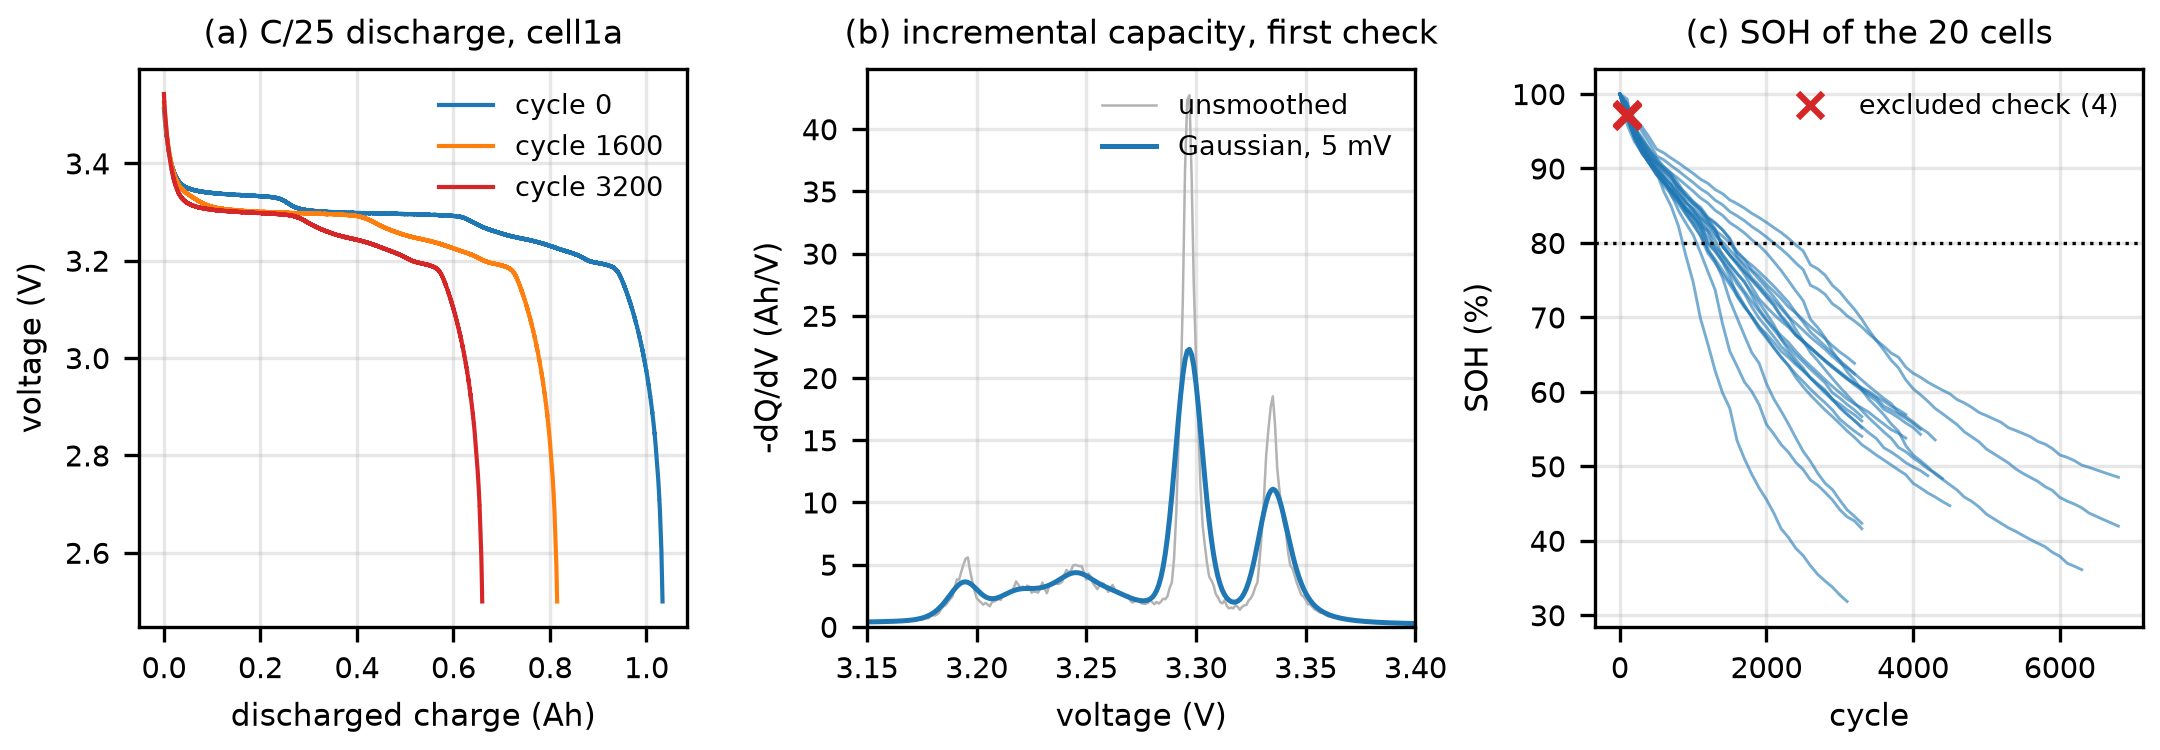
\includegraphics[width=\textwidth]{figures/preprocessing_s6.png}
  \caption{S6 preprocessing (scripts/make\_preprocessing\_figures.py). (a) C/25 discharge of cell 1a at three ages.
    (b) Incremental capacity of its first check without and with the 5~mV Gaussian smoothing used for the IC
    features. (c) SOH of the 20 cells at every valid check; crosses: the four checks excluded by the validity rule,
    placed on the cell's curve at the cycle they were taken (they have no valid capacity). Dotted: 80\% SOH.}
  \label{fig:prep}
\end{figure*}

\begin{figure}[t]
  \centering
  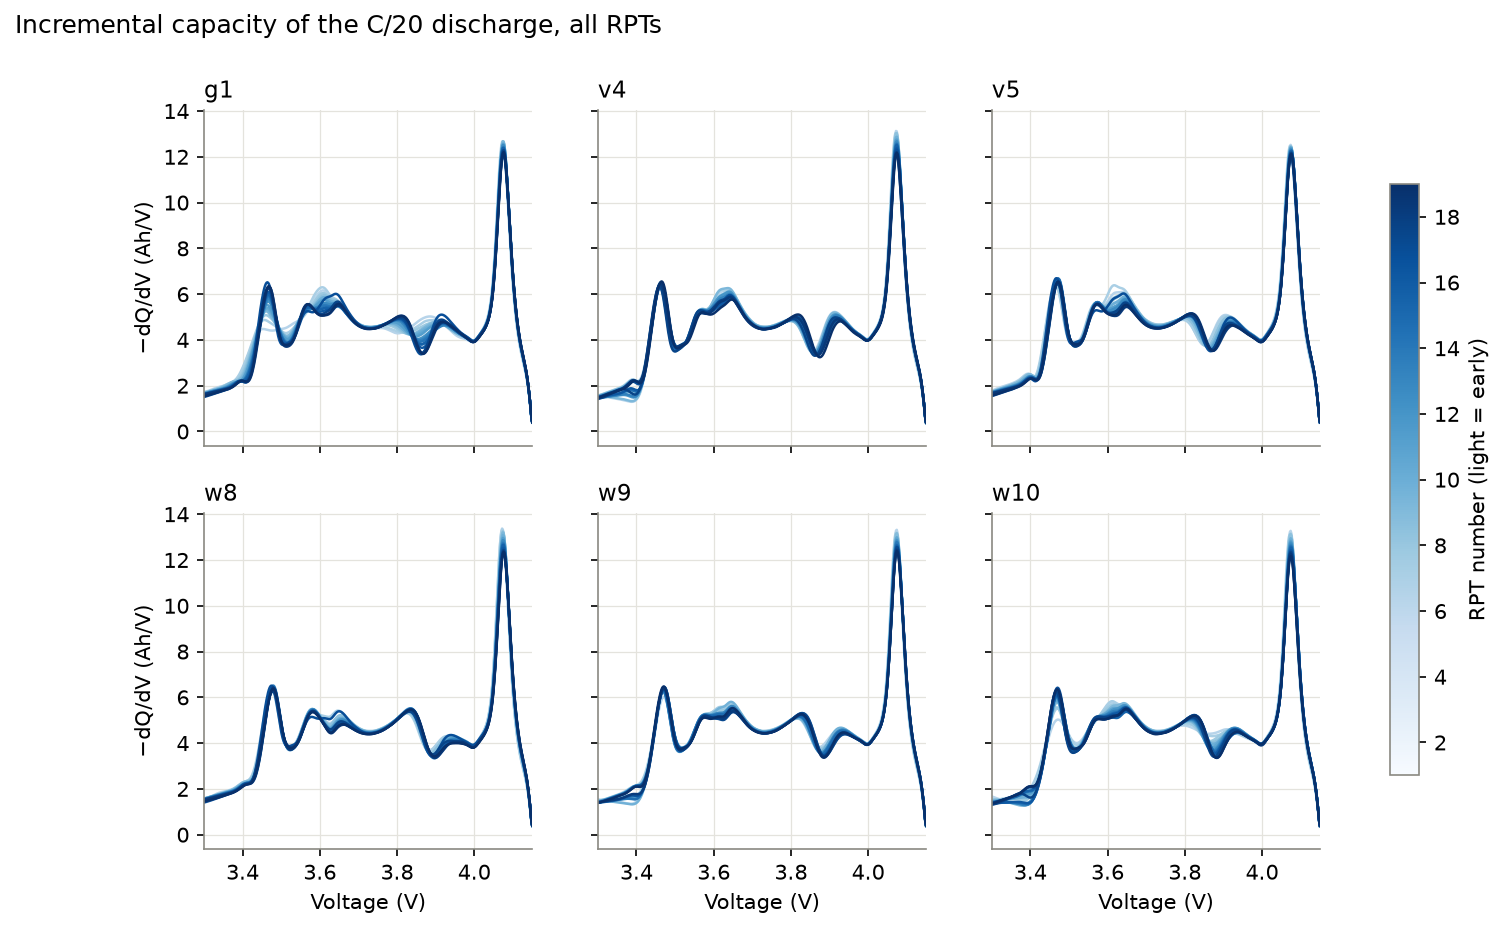
\includegraphics[width=\columnwidth]{figures/11_ic_curves.png}
  \caption{S1: incremental-capacity curves of the C/20 RPTs (10~mV smoothing), notebook 11.}
  \label{fig:ic_s1}
\end{figure}

% -----------------------------------------------------------------------------
\section{Input correlations}

Fig.~\ref{fig:corr} gives the Spearman correlation of the S6 history and diagnostic inputs (F1) with each other and with
the target. Ten of the 17 diagnostics are near-monotone functions of the SOH at the origin ($|\rho|\ge0.9$), so they add little
beyond the SOH history; the fade rate is the input most correlated with the target ($\rho=0.8$). This is consistent
with the ablation in the paper, where removing the diagnostics improved the TFT.

\begin{figure*}[t]
  \centering
  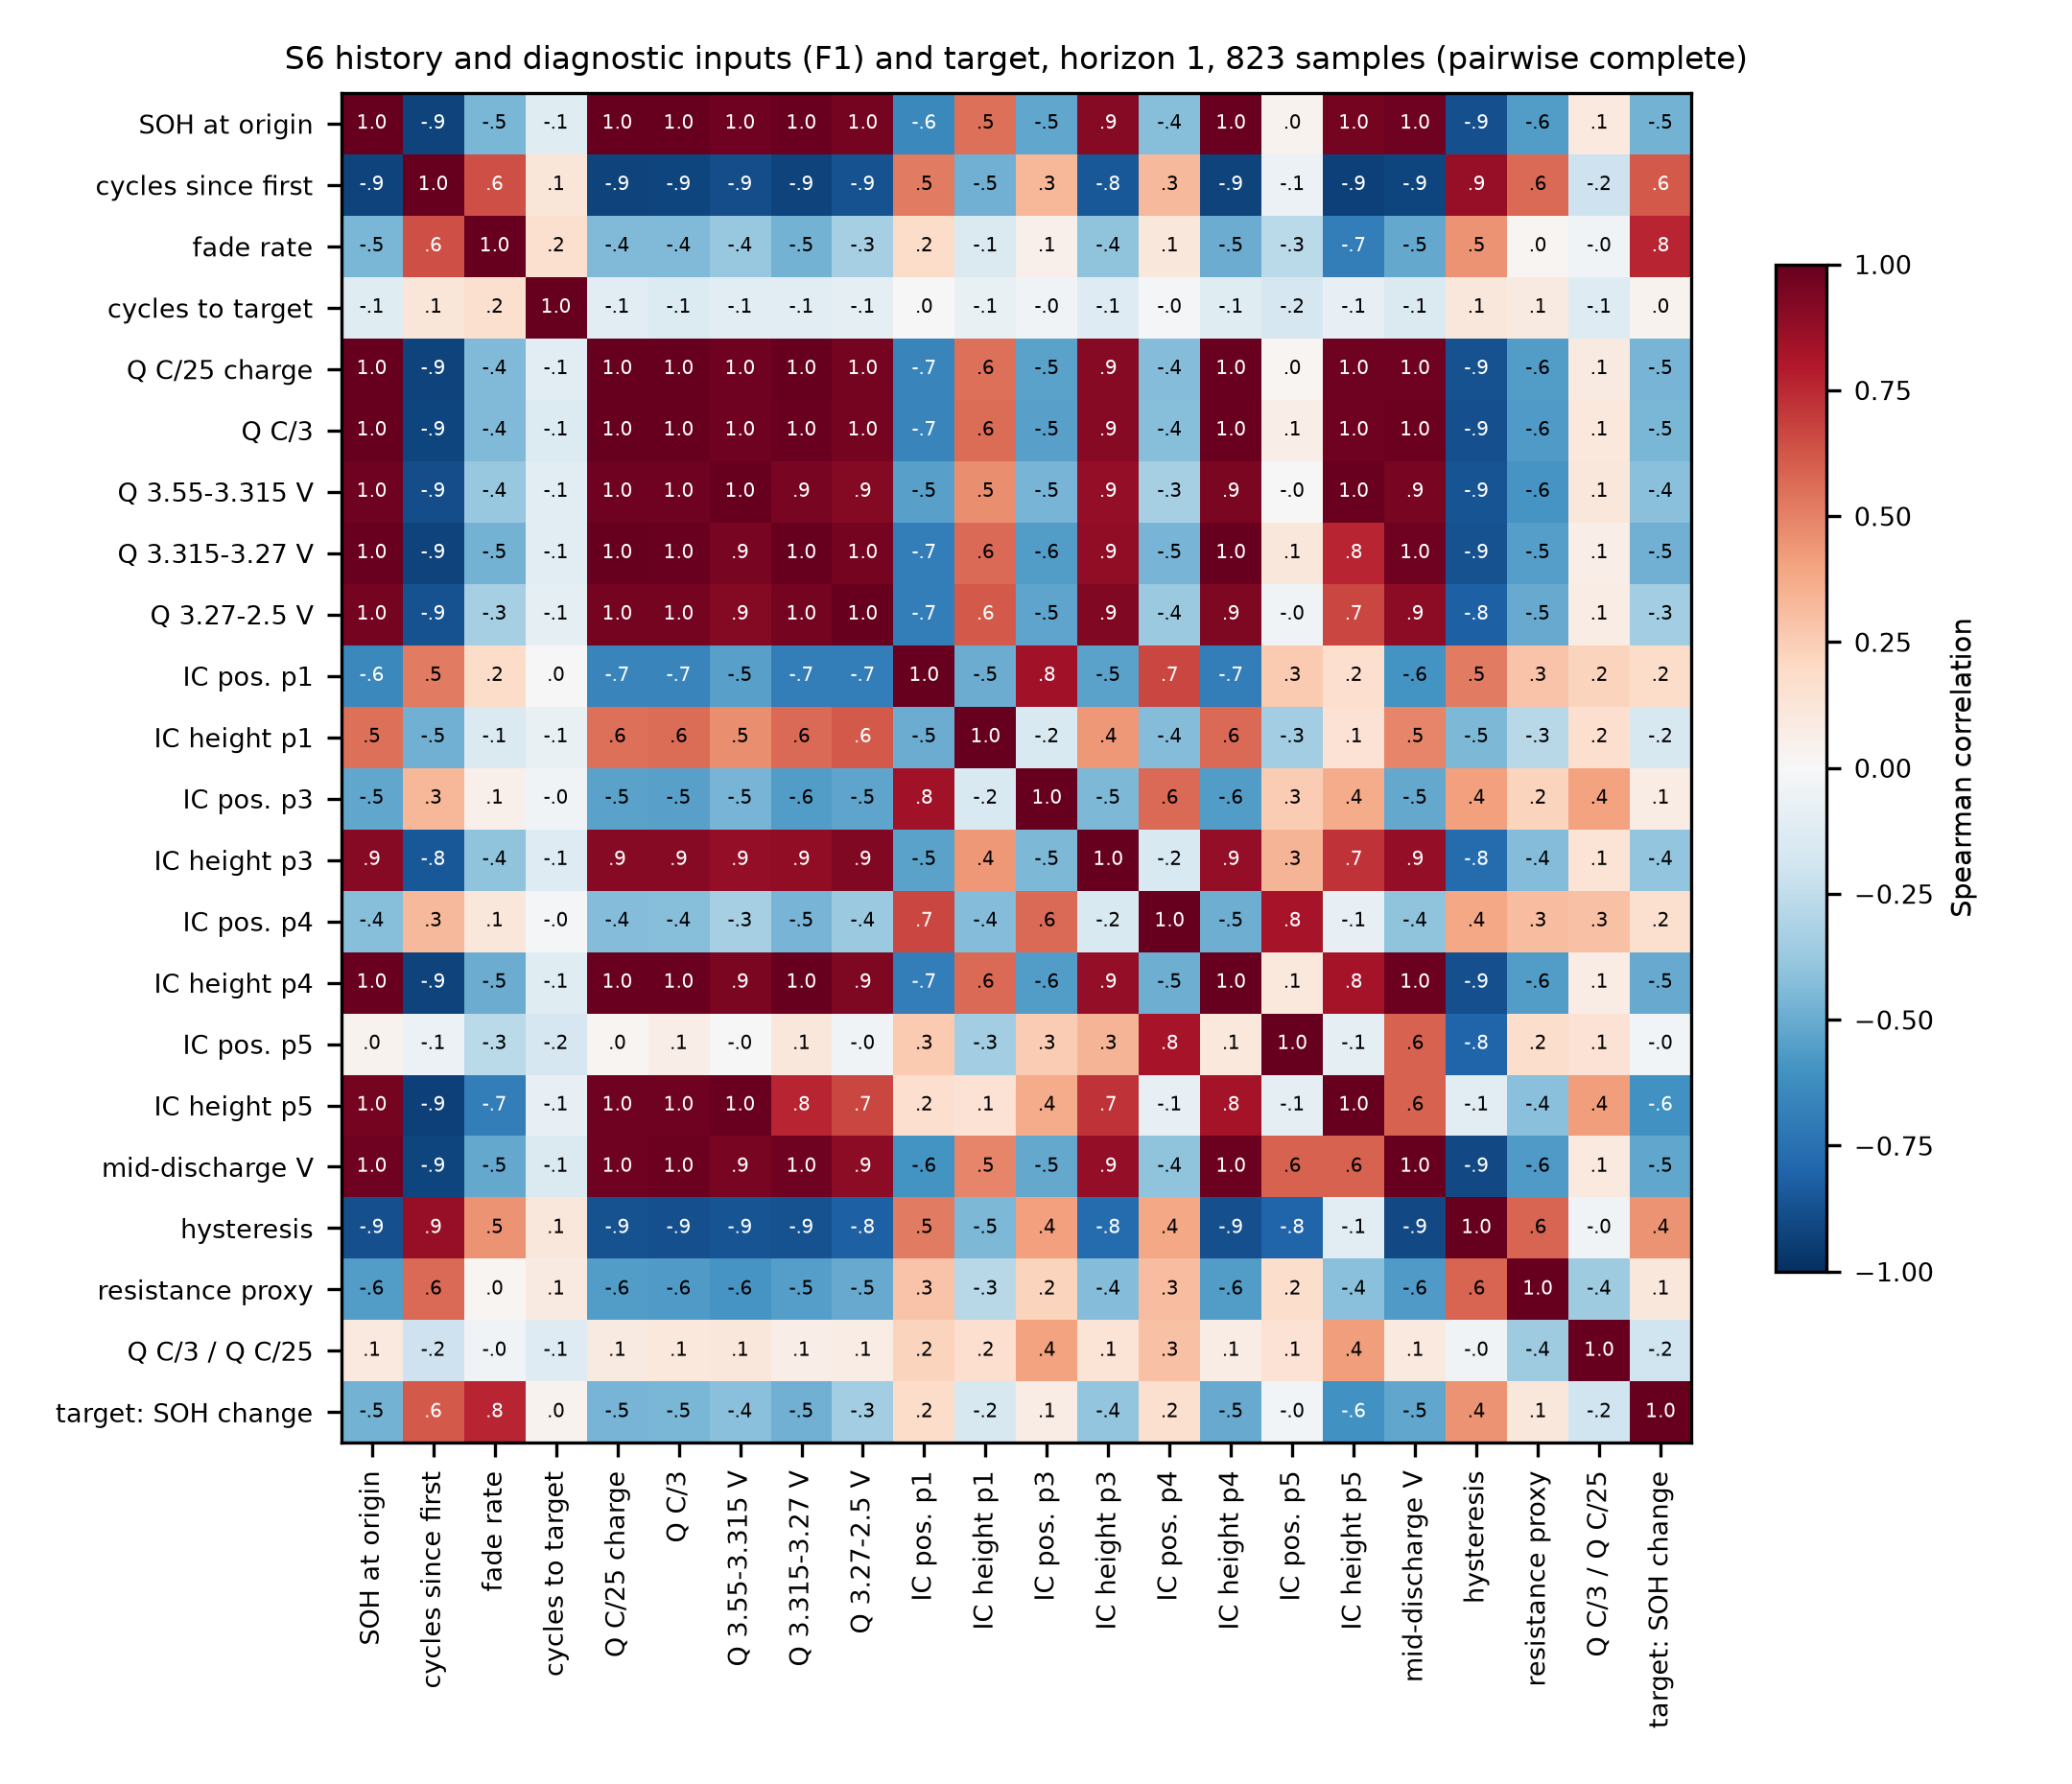
\includegraphics[width=0.82\textwidth]{figures/correlation_s6.png}
  \caption{Spearman correlation of the S6 F1 inputs and the target $\Delta$ (horizon 1, pairwise complete samples;
    the static test conditions are omitted). scripts/make\_preprocessing\_figures.py.}
  \label{fig:corr}
\end{figure*}

% -----------------------------------------------------------------------------
\section{Training curves}

Each task is trained with Adam (batches of 64) for at most 200 epochs, with early stopping on the task's validation
RMSE (patience 20); the weights of the best epoch are kept. Fig.~\ref{fig:epochs} shows one stream of the residual
TFT\,+\,EWC (horizons 1--3, first evaluation order, seed 0, tuned learning rate $3\cdot10^{-3}$ and $\lambda=1$). The
re-run reproduces the committed final average error of that stream exactly (0.464~pp). Validation RMSE reaches its
minimum within 2--30 epochs on five tasks and after 86 epochs on task 6; on task 5 no epoch improved on the
weights carried over from task 4, which were therefore kept.

\begin{figure*}[t]
  \centering
  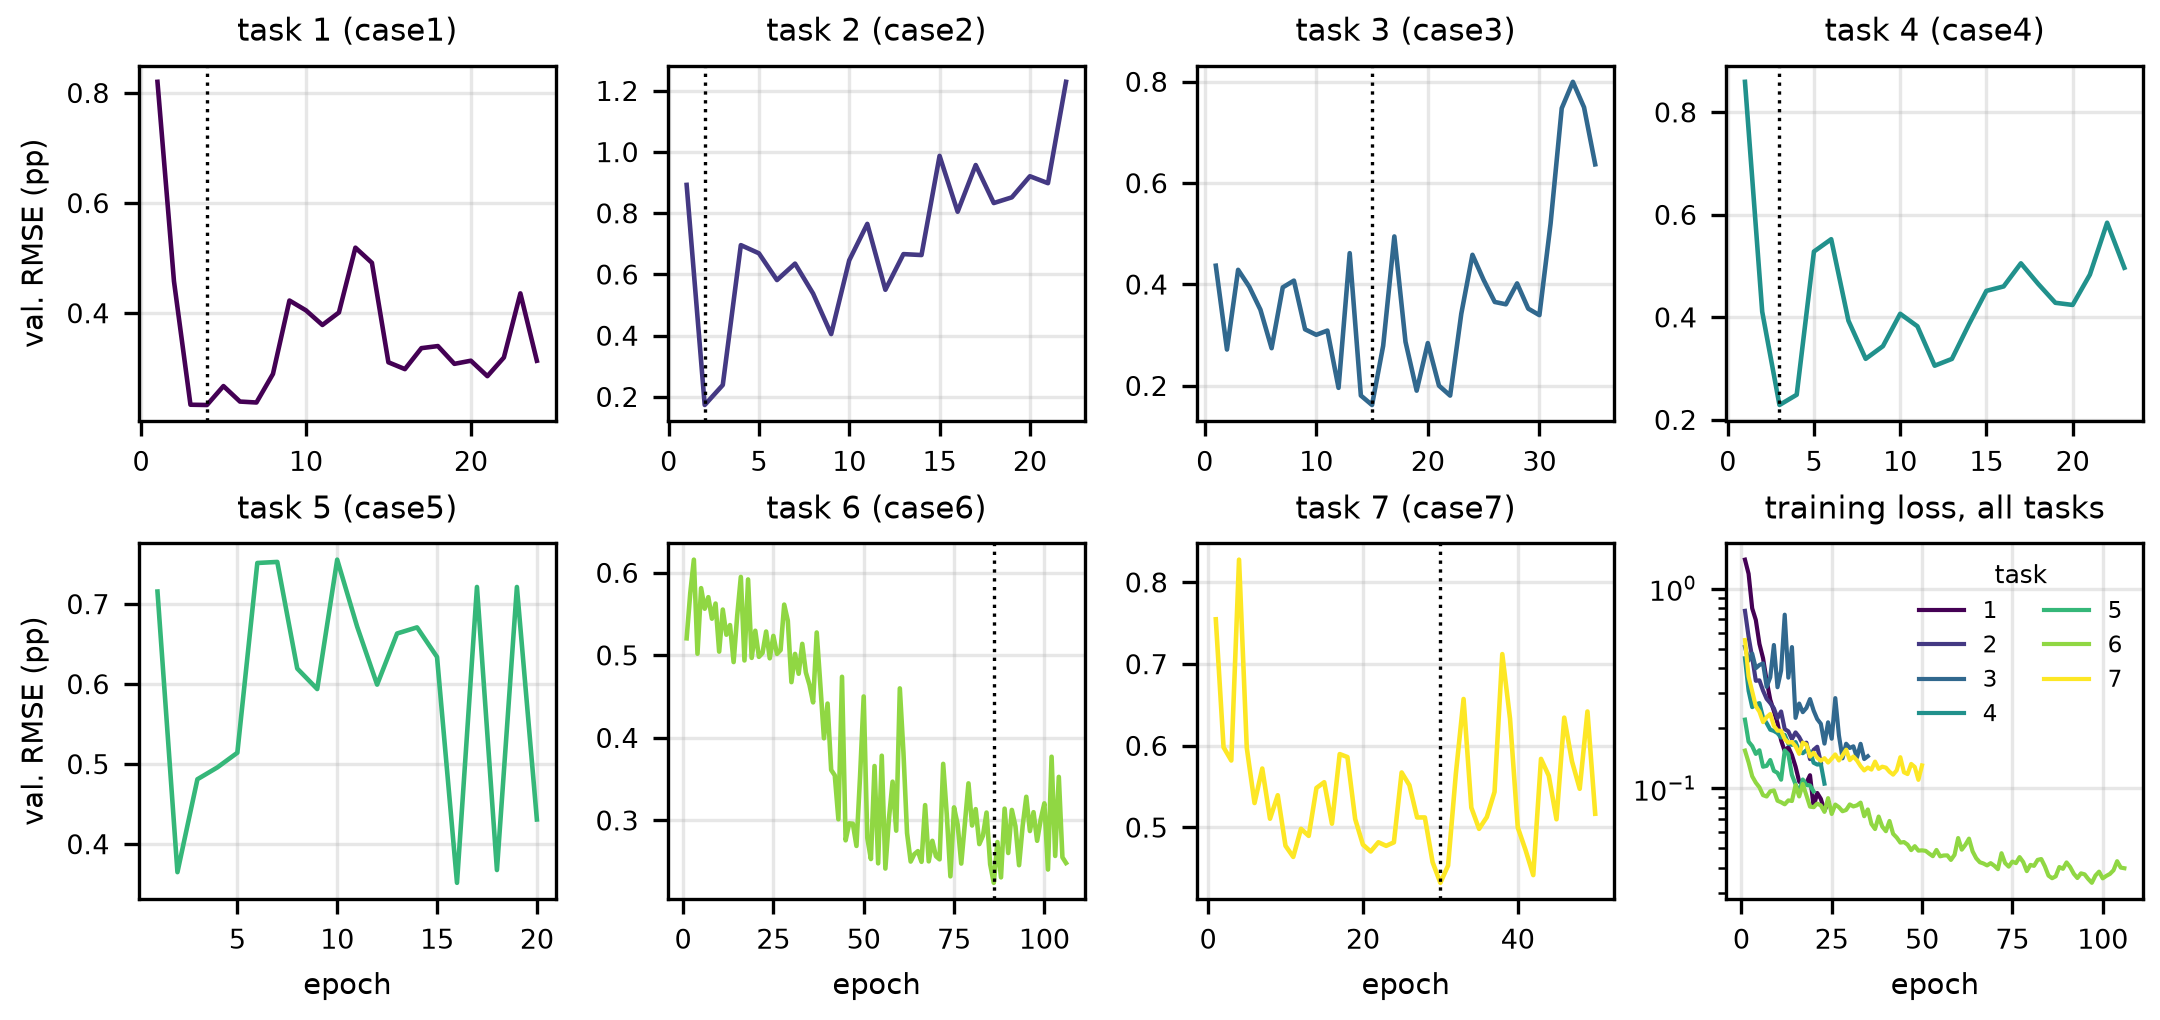
\includegraphics[width=\textwidth]{figures/epoch_curves.png}
  \caption{Residual TFT\,+\,EWC on the S6 stream: validation RMSE per epoch for each task (dotted: early-stopping
    epoch) and training loss (scaled MSE plus EWC penalty) of all tasks. scripts/run\_epoch\_curves.py,
    results/epoch\_curves\_d23\_e1.json.}
  \label{fig:epochs}
\end{figure*}

% -----------------------------------------------------------------------------
\section{Full metric sets (P2)}

Tables~\ref{tab:d30_regression} and \ref{tab:d30_classification} give every regression and classification metric of
the P2 forecasts (decision D30); Fig.~\ref{fig:d30cm} gives the S6 confusion matrices and Fig.~\ref{fig:d30group} the
error per held-out group.

% Generated by scripts/make_d30_outputs.py from results/forecasting_d30_s1.json (commit cb43efb), results/forecasting_d30_s6.json (commit cb43efb)
\begin{table*}[t]
  \centering
  \caption{Protocol P2, all regression metrics of the forecast SOH (pp unless stated), mean over held-out groups (the RMSE column equals Table~\ref{tab:p2} for the baselines; MLP and TFT are re-runs on another platform, within 0.005~pp of it). Bias = mean(forecast $-$ measured): positive values overestimate SOH. NRMSE = RMSE / range of measured SOH in the group. $R^2$ is on the SOH level, $R^2_\Delta$ on the SOH change since the origin (persistence has $R^2_\Delta \le 0$). SOH is relative to the first observed check.}
  \label{tab:d30_regression}
  \setlength{\tabcolsep}{3pt}
  \scriptsize
  \begin{tabular}{llccccccccc}
    \toprule
    Data & Method & RMSE & MSE & MAE & MedAE & Bias & NRMSE & MAPE (\%) & $R^2$ & $R^2_\Delta$ \\
    \midrule
    S1 & Persistence & 0.545 & 0.303 & 0.470 & 0.473 & +0.430 & 0.161 & 0.481 & 0.672 & -1.853 \\
    S1 & Linear extrapolation & 0.511 & 0.293 & 0.365 & 0.226 & -0.014 & 0.148 & 0.374 & 0.690 & -1.314 \\
    S1 & Ridge, usage only & 0.301 & 0.096 & 0.206 & 0.133 & -0.038 & 0.088 & 0.212 & 0.897 & 0.181 \\
    S1 & Ridge, F0 & 0.418 & 0.212 & 0.369 & 0.350 & +0.205 & 0.118 & 0.379 & 0.798 & -0.673 \\
    S1 & Ridge, F1 & 0.320 & 0.115 & 0.266 & 0.241 & +0.065 & 0.092 & 0.273 & 0.881 & 0.083 \\
    S1 & Gradient boosting, F1 & 0.219 & 0.053 & 0.148 & 0.102 & -0.021 & 0.064 & 0.152 & 0.944 & 0.543 \\
    S1 & MLP & 0.285 & 0.087 & 0.211 & 0.162 & +0.009 & 0.083 & 0.216 & 0.907 & 0.260 \\
    S1 & TFT & 0.291 & 0.090 & 0.210 & 0.149 & +0.027 & 0.085 & 0.215 & 0.904 & 0.216 \\
    \midrule
    S6 & Persistence & 2.817 & 8.389 & 2.451 & 2.225 & +2.451 & 0.056 & 3.539 & 0.956 & -3.160 \\
    S6 & Linear extrapolation & 1.372 & 1.946 & 0.738 & 0.333 & +0.050 & 0.028 & 0.973 & 0.988 & -0.050 \\
    S6 & Ridge, usage only & 1.177 & 1.607 & 0.864 & 0.671 & -0.003 & 0.023 & 1.292 & 0.993 & 0.275 \\
    S6 & Ridge, F0 & 0.859 & 0.905 & 0.613 & 0.439 & +0.028 & 0.016 & 0.893 & 0.996 & 0.614 \\
    S6 & Ridge, F1 & 1.137 & 1.767 & 0.749 & 0.550 & +0.013 & 0.022 & 1.130 & 0.991 & 0.221 \\
    S6 & Gradient boosting, F1 & 0.710 & 0.725 & 0.488 & 0.321 & +0.097 & 0.013 & 0.710 & 0.997 & 0.736 \\
    S6 & MLP & 0.826 & 1.018 & 0.608 & 0.444 & +0.220 & 0.015 & 0.914 & 0.996 & 0.656 \\
    S6 & TFT & 0.868 & 1.151 & 0.621 & 0.424 & +0.235 & 0.016 & 0.928 & 0.996 & 0.622 \\
    \bottomrule
  \end{tabular}
\end{table*}


% Generated by scripts/make_d30_outputs.py from results/forecasting_d30_s1.json (commit cb43efb), results/forecasting_d30_s6.json (commit cb43efb)
\begin{table*}[t]
  \centering
  \caption{Protocol P2, reuse class (C0--C3, D10 cut-points) and end-of-first-life decision (SOH $\le$ 80, positive) of the forecast SOH against the measured SOH, all held-out samples pooled (mean over seeds). Macro averages run over the measured classes. AUC uses the forecast SOH as the score (point forecasts; no class probabilities, so no log loss). Measured class counts of all samples: S1: C0 279, C1 0, C2 0, C3 0; S6: C0 52, C1 182, C2 516, C3 1659. -- : undefined (one class only).}
  \label{tab:d30_classification}
  \setlength{\tabcolsep}{3pt}
  \scriptsize
  \begin{tabular}{llccccccccccccccc}
    \toprule
    Data & Method & Acc. & Bal. acc. & Prec. & Rec. & Spec. & F1 & MCC & $\kappa$ & $\kappa_w$ & EoL Prec. & EoL Rec. & EoL Spec. & EoL F1 & EoL MCC & EoL AUC \\
    \midrule
    S1 & Persistence & 1.00 & 1.00 & 1.00 & 1.00 & -- & 1.00 & -- & -- & -- & -- & -- & 1.00 & -- & -- & -- \\
    S1 & Linear extrapolation & 0.98 & 0.98 & 1.00 & 0.98 & -- & 0.99 & -- & 0.00 & 0.00 & -- & -- & 1.00 & -- & -- & -- \\
    S1 & Ridge, usage only & 1.00 & 1.00 & 1.00 & 1.00 & -- & 1.00 & -- & 0.00 & 0.00 & -- & -- & 1.00 & -- & -- & -- \\
    S1 & Ridge, F0 & 1.00 & 1.00 & 1.00 & 1.00 & -- & 1.00 & -- & -- & -- & -- & -- & 1.00 & -- & -- & -- \\
    S1 & Ridge, F1 & 1.00 & 1.00 & 1.00 & 1.00 & -- & 1.00 & -- & -- & -- & -- & -- & 1.00 & -- & -- & -- \\
    S1 & Gradient boosting, F1 & 0.99 & 0.99 & 1.00 & 0.99 & -- & 0.99 & -- & 0.00 & 0.00 & -- & -- & 1.00 & -- & -- & -- \\
    S1 & MLP & 1.00 & 1.00 & 1.00 & 1.00 & -- & 1.00 & -- & 0.00 & 0.00 & -- & -- & 1.00 & -- & -- & -- \\
    S1 & TFT & 1.00 & 1.00 & 1.00 & 1.00 & -- & 1.00 & -- & 0.00 & 0.00 & -- & -- & 1.00 & -- & -- & -- \\
    \midrule
    S6 & Persistence & 0.86 & 0.78 & 0.62 & 0.78 & 0.96 & 0.66 & 0.72 & 0.72 & 0.81 & 1.00 & 0.93 & 1.00 & 0.96 & 0.89 & 1.00 \\
    S6 & Linear extrapolation & 0.94 & 0.84 & 0.81 & 0.84 & 0.98 & 0.78 & 0.88 & 0.87 & 0.91 & 1.00 & 0.98 & 0.99 & 0.99 & 0.96 & 1.00 \\
    S6 & Ridge, usage only & 0.95 & 0.91 & 0.83 & 0.91 & 0.98 & 0.85 & 0.90 & 0.90 & 0.93 & 0.99 & 0.98 & 0.98 & 0.99 & 0.96 & 1.00 \\
    S6 & Ridge, F0 & 0.96 & 0.88 & 0.89 & 0.88 & 0.99 & 0.88 & 0.92 & 0.92 & 0.94 & 1.00 & 0.98 & 0.99 & 0.99 & 0.97 & 1.00 \\
    S6 & Ridge, F1 & 0.96 & 0.84 & 0.88 & 0.84 & 0.98 & 0.85 & 0.91 & 0.91 & 0.93 & 0.99 & 0.99 & 0.97 & 0.99 & 0.96 & 1.00 \\
    S6 & Gradient boosting, F1 & 0.97 & 0.89 & 0.89 & 0.89 & 0.99 & 0.89 & 0.93 & 0.93 & 0.95 & 0.99 & 0.99 & 0.98 & 0.99 & 0.97 & 1.00 \\
    S6 & MLP & 0.96 & 0.86 & 0.88 & 0.86 & 0.99 & 0.87 & 0.92 & 0.92 & 0.94 & 0.99 & 0.99 & 0.98 & 0.99 & 0.97 & 1.00 \\
    S6 & TFT & 0.96 & 0.88 & 0.89 & 0.88 & 0.99 & 0.88 & 0.92 & 0.92 & 0.94 & 0.99 & 0.98 & 0.99 & 0.99 & 0.96 & 1.00 \\
    \bottomrule
  \end{tabular}
\end{table*}


\begin{figure*}[t]
  \centering
  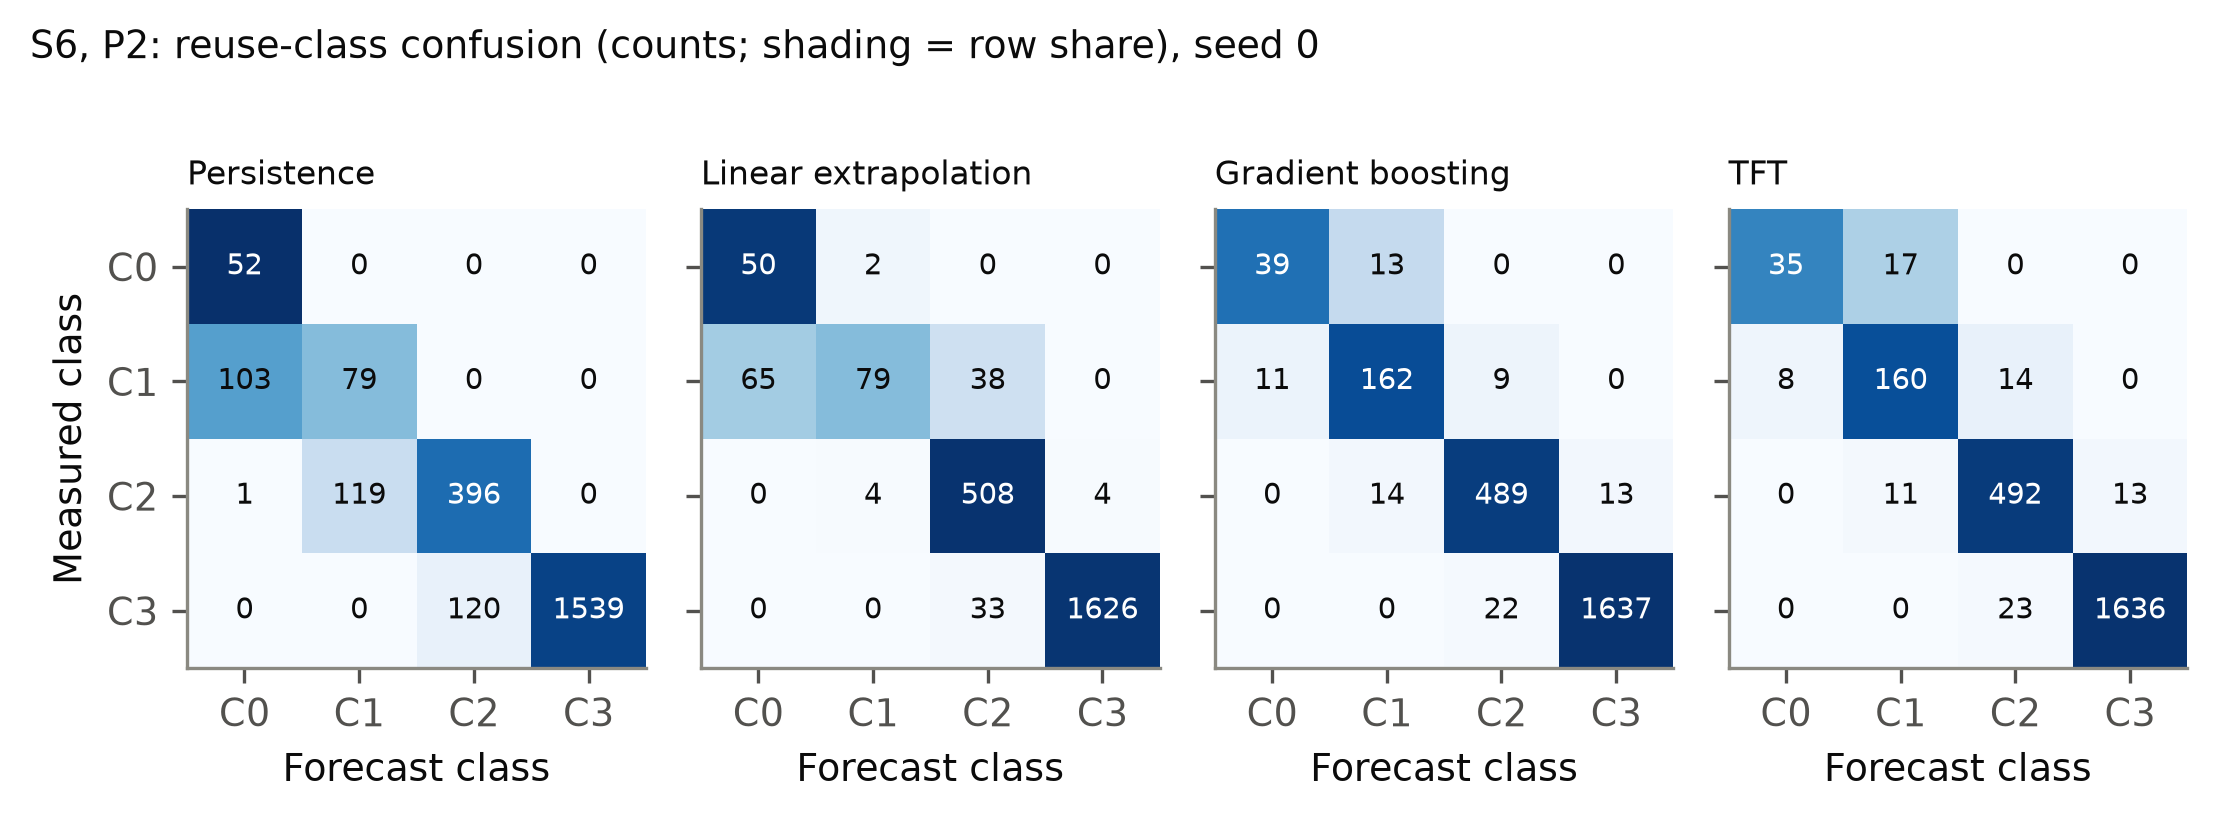
\includegraphics[width=\textwidth]{figures/d30_confusion.png}
  \caption{S6, P2: reuse-class confusion matrices (counts; shading: row share), seed 0. scripts/make\_d30\_outputs.py.}
  \label{fig:d30cm}
\end{figure*}

\begin{figure*}[t]
  \centering
  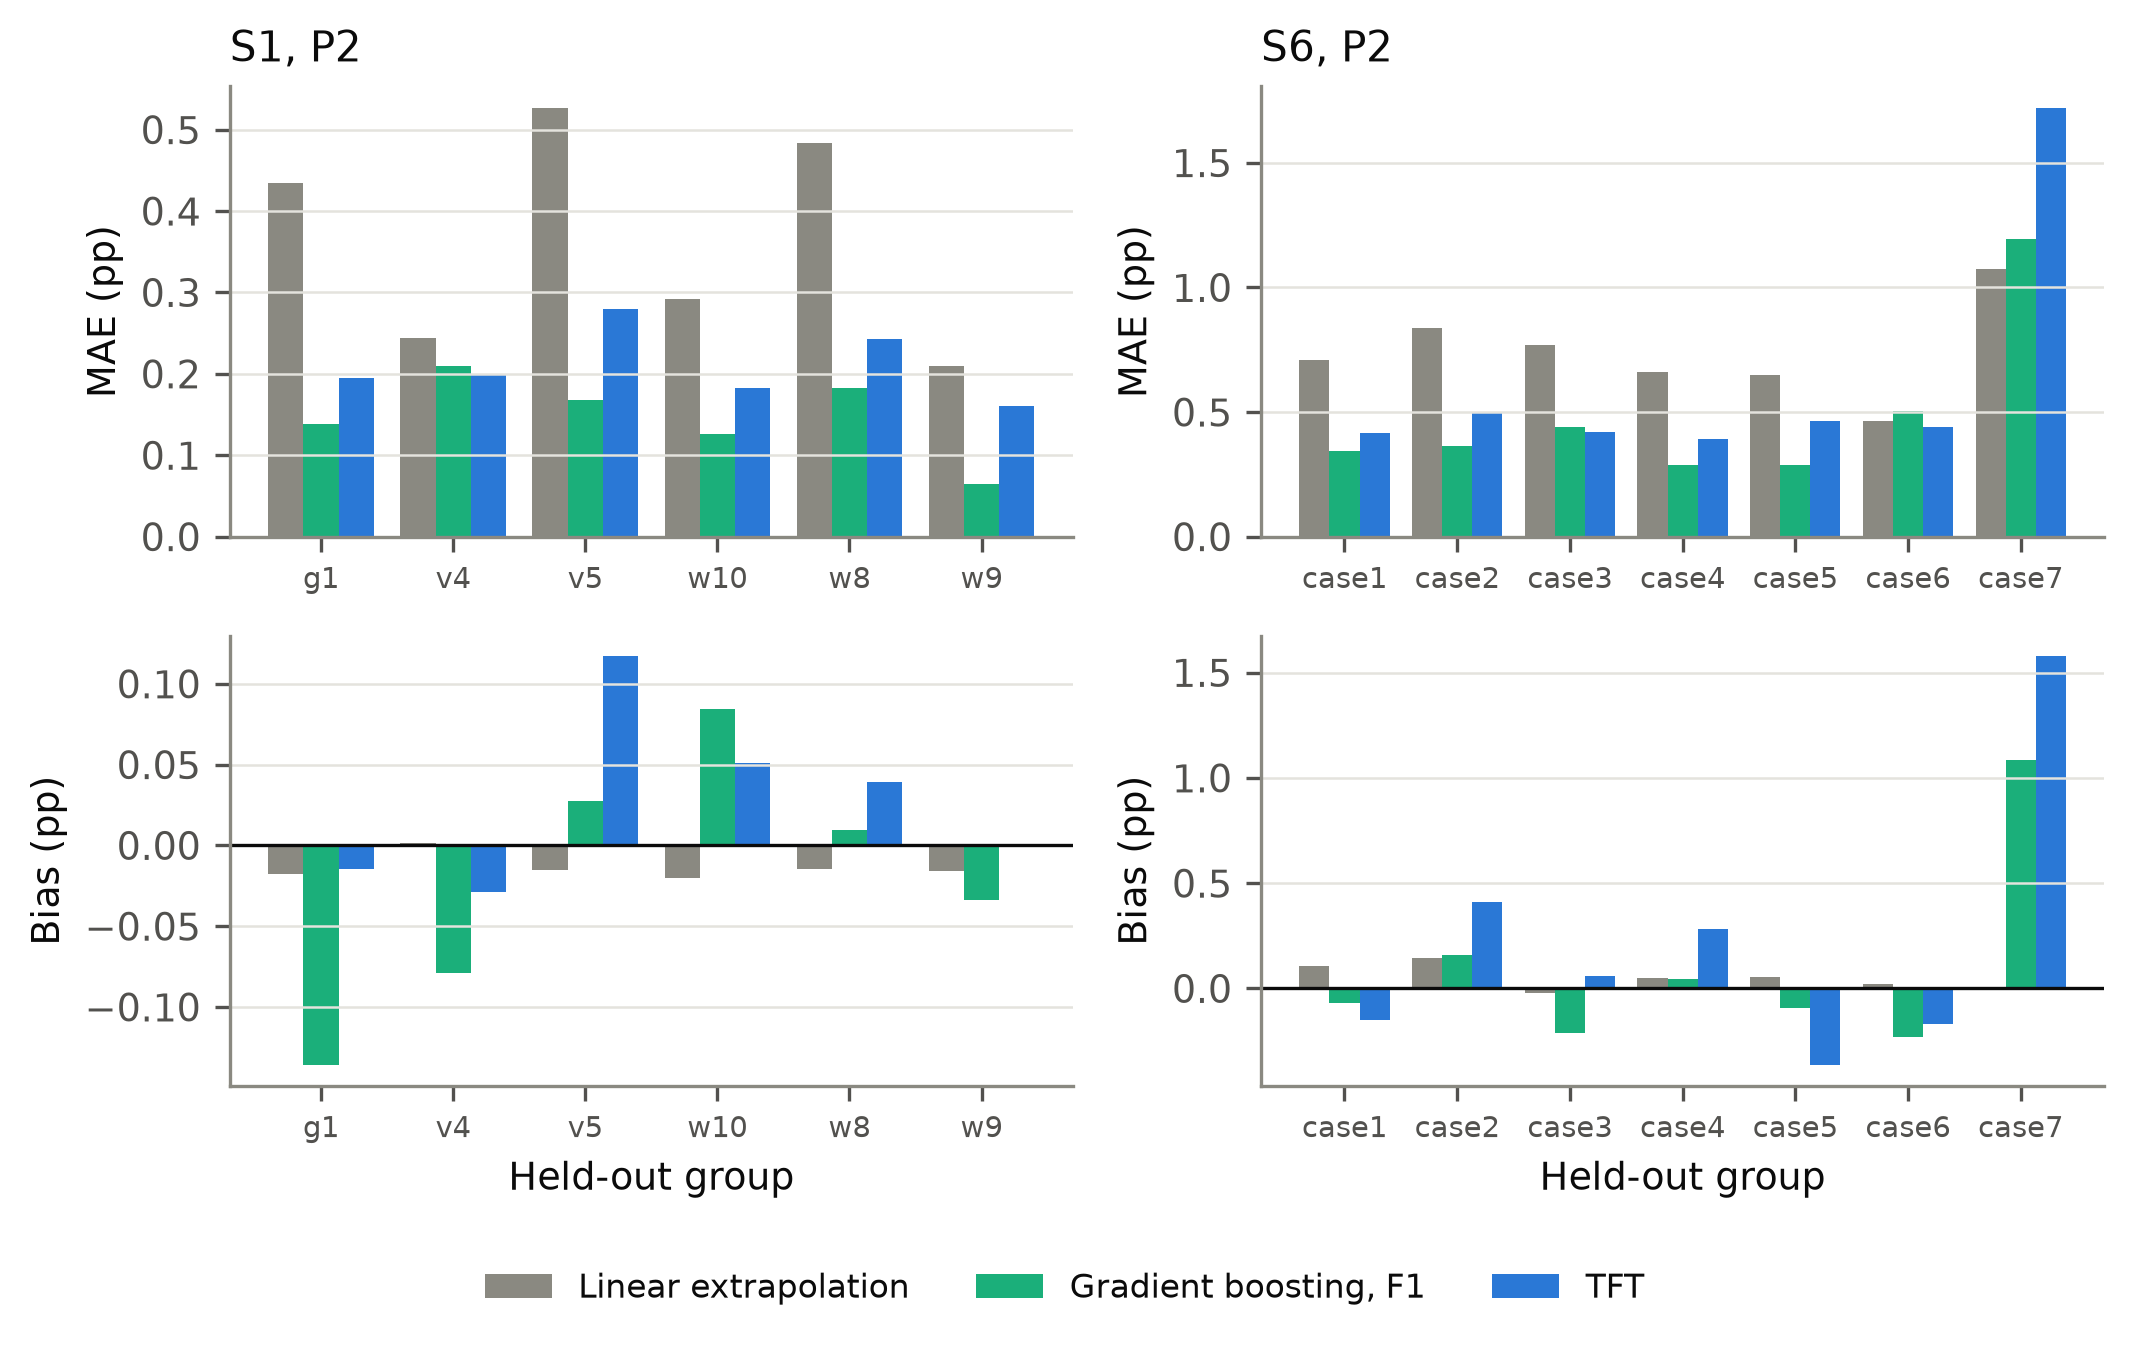
\includegraphics[width=\textwidth]{figures/d30_error_by_group.png}
  \caption{P2: error per held-out group. scripts/make\_d30\_outputs.py.}
  \label{fig:d30group}
\end{figure*}

% -----------------------------------------------------------------------------
\section{Ageing-cycle processing and first-life pretraining}

\emph{Spark job.} Between checks, every S6 cell logged each ageing cycle at about one sample per second: 827 files,
132~GB raw and $9.0\times10^{8}$ rows. Apache Spark~4.2 (PySpark, local mode) reduces them to block-level inputs: one map
task per 100-cycle block derives, for every cycle, a validity flag and seven measured responses (end-of-charge and
end-of-discharge voltage, constant-voltage hold time and final current, relaxation after charge and after discharge,
internal resistance); Spark SQL groups the cached per-cycle table (82{,}529 cycles) by cell and block into the mean,
last value and slope of each response (21 inputs), and each block joins the origin at the check that ends it. Charge,
energy and current are excluded because the protocol scales them with the previous capacity (within-cell
$r=0.97$--$0.999$ with the previous check's capacity). The run takes 20~min on six cores and matches an independent
pandas implementation on all 827 blocks (largest difference $2\times10^{-13}$).

\emph{First-life pretraining (P3).} The pool provides 36{,}711 samples, against 2{,}409 in S6, and validation selected
EWC $\lambda=0.01$ for the pretrained TFT. Under the replication rule, EWC and fine-tuning are practically equivalent for
the pretrained TFT (differences of 0.015--0.017~pp). The S6 stream does not degrade the pool test error
(TFT\,+\,EWC: 3.280 to 3.148~pp), but on that split the pretrained models are also less accurate than extrapolation
(3.001~pp): pretraining does not learn a first-life model worth transferring.

\emph{Attention.} The TFT's attention over the four previous origins is nearly uniform (0.24--0.26 per lag): it makes
little use of its history.

% -----------------------------------------------------------------------------
\section{Additional results}

Table~\ref{tab:residual} and Figs.~\ref{fig:d25} and \ref{fig:d27} belong to Sections IV-D to IV-G of the paper and
were moved here for space.

\emph{Reproducibility of the comparisons (Section IV-B).} P1 and P2 were re-run in a pinned environment on data rebuilt from the raw archives. Every baseline, every P2 result and the ranking of methods reproduced; the neural models moved by at most 0.059~pp. On S1, five Holm-corrected comparisons with TFT\,+\,EWC crossed $p=0.05$. On S6, validation selected EWC $\lambda=1000$ instead of 100 (a 0.008~pp tie), and the error advantage of TFT\,+\,EWC over fine-tuning moved from $p_{\mathrm{Holm}}=0.005$ to 0.060, while its reduction of forgetting moved from 0.050 to 0.008. These findings motivated the ten tuning orders, the one-standard-error rule and the replication rule used from P3 on. A D30 re-run of P2 on another platform reproduced every baseline exactly and moved the MLP and TFT by at most 0.027~pp per held-out group: neural training is deterministic per platform, not across platforms.

\emph{Reuse classes in the D30 re-run of P2.} On S6 the learned models assign the measured reuse class to 95--97\% of samples (MCC 0.90--0.93), against 94\% (0.88) for linear extrapolation and 86\% (0.72) for persistence, and all errors but one (persistence) are between neighbouring classes; the end-of-first-life decision does not separate the methods (AUC $\ge$0.998), as 69\% of S6 samples are below 80\%.

\emph{Intervals on unseen conditions.} Intervals (Fig.~\ref{fig:d27}) calibrated on the pooled validation rows of the training conditions under-cover on the held-out one, for the TFT (pooled 0.66--0.68) and for extrapolation (0.74--0.76) alike. Calibrating extrapolation, which has no fitted parameters, on all origins of those conditions instead of their mid-life validation rows restores 0.89--0.90: the calibration rows caused the shortfall, not only the model. With leave-one-condition-out calibration, gradient-boosting intervals reach the registered threshold of 0.85 (0.90 in both horizon sets) with the lowest mean interval scores (3.2 and 6.7~pp, against 7.1 and 11.8~pp for calibrated extrapolation and 6.1--6.3 and 10.0--10.3~pp for the TFT), lower than calibrated extrapolation's on six of seven conditions (significant only for horizons 1--3, $p=0.047$, against $p=0.30$, so not established). Coverage holds over conditions, not for each: on the 100\% depth-of-discharge condition, outside the range of the others, it is 0.48 and 0.38.

The paper's table of errors on unseen conditions (Section IV-G) lists the shrunk residual TFT\,+\,EWC; the raw correction gives 0.88/0.90, 0.79/0.80, 1.59/1.62 and 1.46/1.49~pp in the same columns.

\begin{table}[t]
  \centering
  \caption{Learned residual, shift-adaptive EWC and literature baselines on S6 (stream from scratch): final average test RMSE (pp), mean over 50 runs, main / replicate seed sets, and forgetting (pp) for horizons 1--6. Below the line: single fits on all tasks (not continual) and extrapolation.}
  \label{tab:residual}
  \setlength{\tabcolsep}{2.5pt}
  \scriptsize
  \begin{tabular}{lccc}
    \toprule
    Method & E1: $h{=}1$--3 & E2: $h{=}1$--6 & Forgetting, E2 \\
    \midrule
    \textbf{TFT\,+\,EWC, residual} & \textbf{0.339 / 0.314} & \textbf{0.561 / 0.534} & \textbf{0.093 / 0.086} \\
    TFT\,+\,SA-EWC, residual & 0.343 / 0.321 & 0.548 / 0.564 & 0.066 / 0.084 \\
    TFT fine-tuning, residual & 0.347 / 0.337 & 0.673 / 0.612 & 0.282 / 0.220 \\
    TFT\,+\,EWC, direct & 0.504 / 0.487 & 0.802 / 0.835 & 0.135 / 0.166 \\
    MLP\,+\,EWC, residual & 0.374 / 0.366 & 0.659 / 0.694 & 0.205 / 0.225 \\
    BiLSTM\,+\,EWC, residual & 0.328 / 0.370 & 0.669 / 0.765 & 0.229 / 0.318 \\
    Transformer\,+\,EWC, residual & 0.360 / 0.366 & 0.609 / 0.705 & 0.129 / 0.198 \\
    TCN\,+\,EWC, residual & 0.466 / 0.408 & 0.812 / 0.756 & 0.345 / 0.268 \\
    \midrule
    Linear extrapolation & 0.343 & 0.485 & -- \\
    Gradient boosting & 0.451 & 0.898 & -- \\
    SVR, residual & 0.429 & 0.616 & -- \\
    GPR, direct & 1.374 & 2.073 & -- \\
    \bottomrule
  \end{tabular}
\end{table}

\begin{figure}[t]
  \centering
  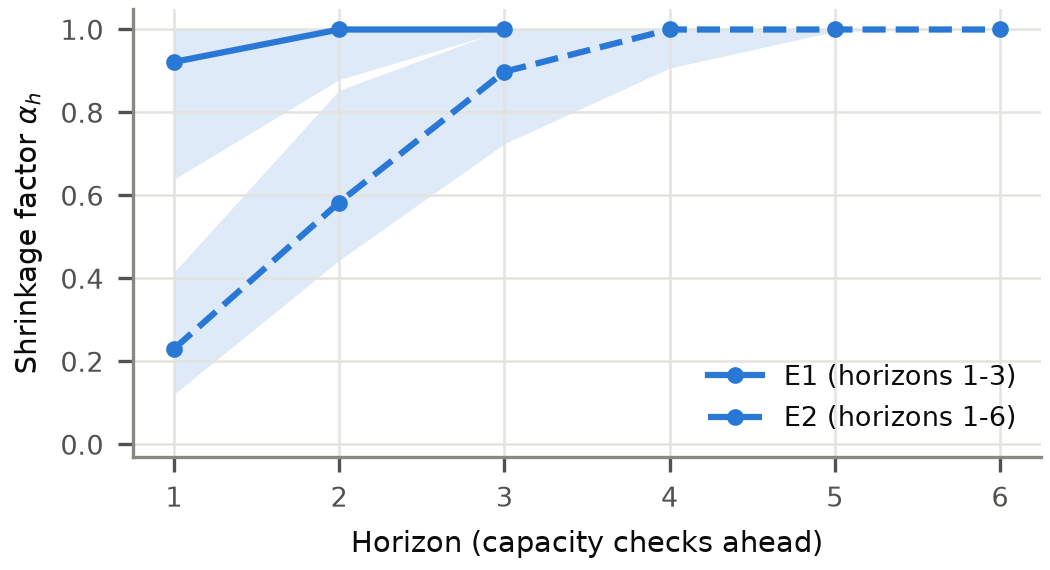
\includegraphics[width=\columnwidth]{figures/d25_shrinkage.png}
  \caption{S6 stream: shrinkage factor $\alpha_h$ of the TFT correction per horizon after the last task (median and interquartile range over 50 runs, seeds 0--4); $\alpha_h=0$ is linear extrapolation.}
  \label{fig:d25}
\end{figure}

\begin{figure}[t]
  \centering
  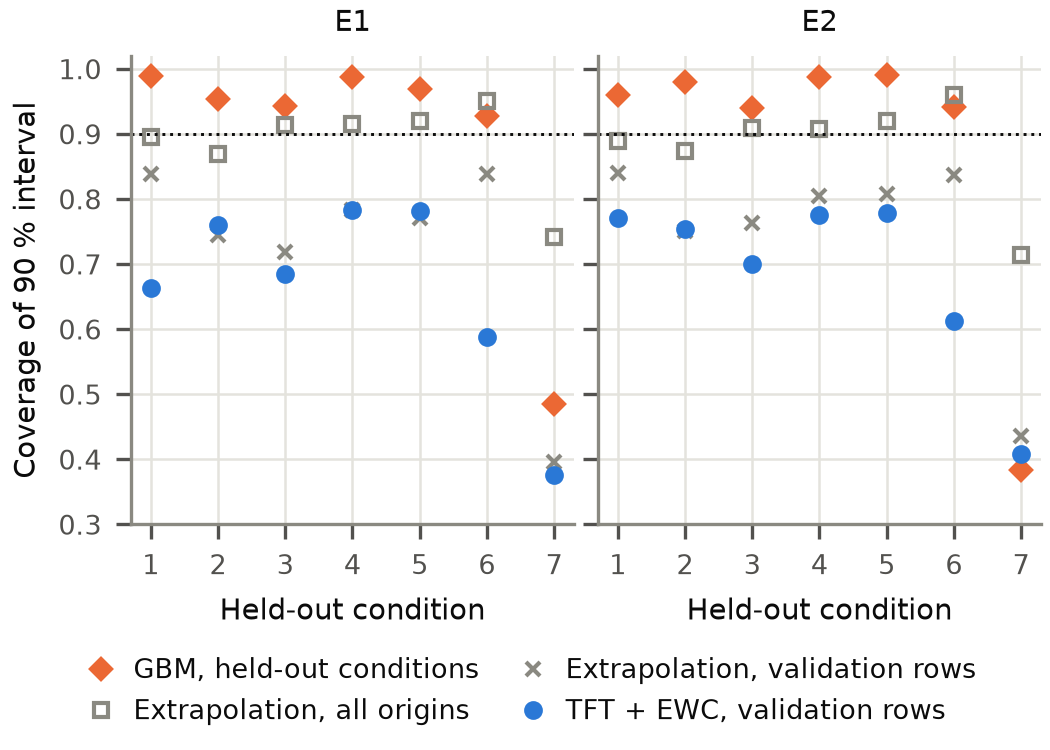
\includegraphics[width=\columnwidth]{figures/d27_coverage.png}
  \caption{Unseen S6 conditions: coverage of 90\% conformal intervals per held-out condition, by forecaster and calibration rows. TFT: mean over 50 runs (seeds 0--4). Dotted: nominal level.}
  \label{fig:d27}
\end{figure}

\end{document}
